\documentclass{standalone}
\usepackage{tikz}
\usepackage{standalone}
\begin{document}
	
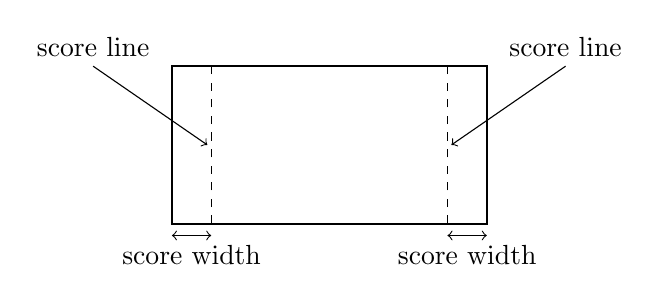
\begin{tikzpicture}
%\draw [help lines] (-3,-2) grid (8,4);

\draw [<->] (0,-.15) -- (0.5,-.15);
\draw [<->] (3.5,-.15) -- (4,-.15);

\draw [->] (-1,2) -- (0.45,1);
\draw [->] (5,2) -- (3.55,1);

\node at (-1,2.25) {score line};
\node at (5,2.25) {score line};
\node at (0.25,-.4) {score width};
\node at (3.75,-.4) {score width};

\draw [thick] (0,0) rectangle (4,2);
\draw [dashed] (0.5,0) -- (0.5,2);
\draw [dashed] (3.5,0) -- (3.5,2);


\end{tikzpicture}
	
\end{document}